%\documentclass{beamer}
%\usetheme{Pittsburgh}
\documentclass{scrartcl}

\usepackage[utf8]{inputenc}
\usepackage{default}
\usepackage[procnames]{listings}
\usepackage{graphicx}
%\usepackage[toc,page]{appendix}
\usepackage{caption}
\usepackage{hyperref}
\usepackage{color}
%\usepackage{csvsimple}
\usepackage{float}
\usepackage[T1]{fontenc}



%Bibliogrpahy?
\usepackage{bibentry}
%\nobibliography*
%\bibentry{ }


%Python
\definecolor{keywords}{RGB}{255,0,90}
\definecolor{comments}{RGB}{0,0,113}
\definecolor{red}{RGB}{160,0,0}
\definecolor{green}{RGB}{0,150,0}
\lstset{language=Python,
    basicstyle=\ttfamily\scriptsize,
    keywordstyle=\color{keywords},
    commentstyle=\color{comments},
    stringstyle=\color{red},
    identifierstyle=\color{green},
    breaklines = true,
    columns=fullflexible,
    %Numbering and tabs
    %numbers=left,
    %numberstyle=\tiny\color{gray},
    %stepnumber=2,
    %numbersep=1em,
    tabsize=4,
    showspaces=false,
    showstringspaces=false}

\begin{document}

\title{Scientific Experimentation and Evaluation
}
\subtitle{
Assignment: 5}
\author{
  Quignon, Christophe\\
  Matin, Maryam
  %Familyname, Name
}
\date{\today}


\maketitle


\section{Experiment}
To assure a reliable motion model for this week's assignment, we decided to repeat the recordings. This time we avoided recording at the intersection of two cameras and used a bigger marker to ensure the robot is traceable even in the farthest distance relative to the camera. To make the measurements more accurate and reduce the outliers at the end position we flip the marker and stop recording at the same time .  



\subsection{Data representation}
Figures 1 to 3 show the plotted trajectories for each of the runs in cartesian coordinates. As depicted in the in figures, there are a number of outliers at the beginning and ending of each path which are most likely caused by flipping the marker up and down at these points.


\begin{figure}[H]
\centering
\begin{minipage}{.5\textwidth}
  \centering
  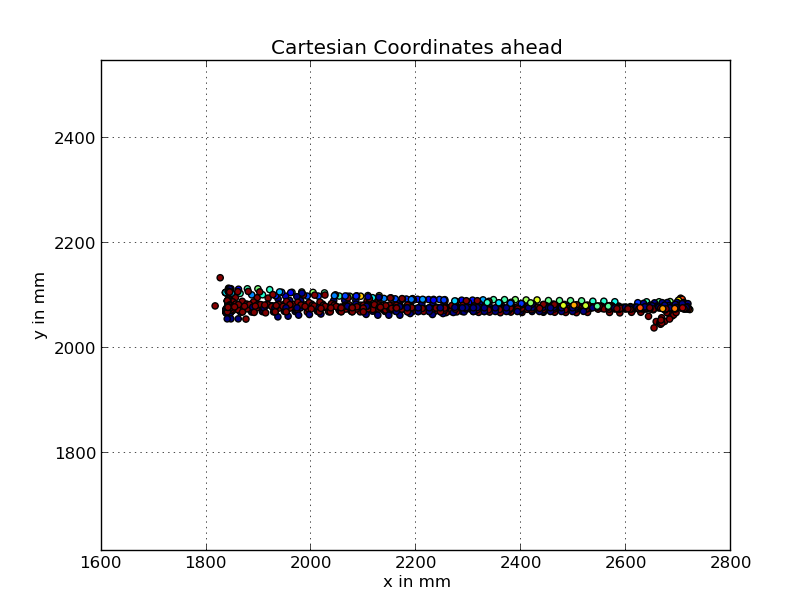
\includegraphics[width=1\linewidth]{img_second_run/Cartesian_ahead.png}
  %\caption{}
  %\label{fig:}
\end{minipage}%

\caption{Recordings of the ahead movements in cartesian coordinates.}
\label{fig:outliers}
\end{figure}


\begin{figure}[H]
\centering
\begin{minipage}{.5\textwidth}
  \centering
  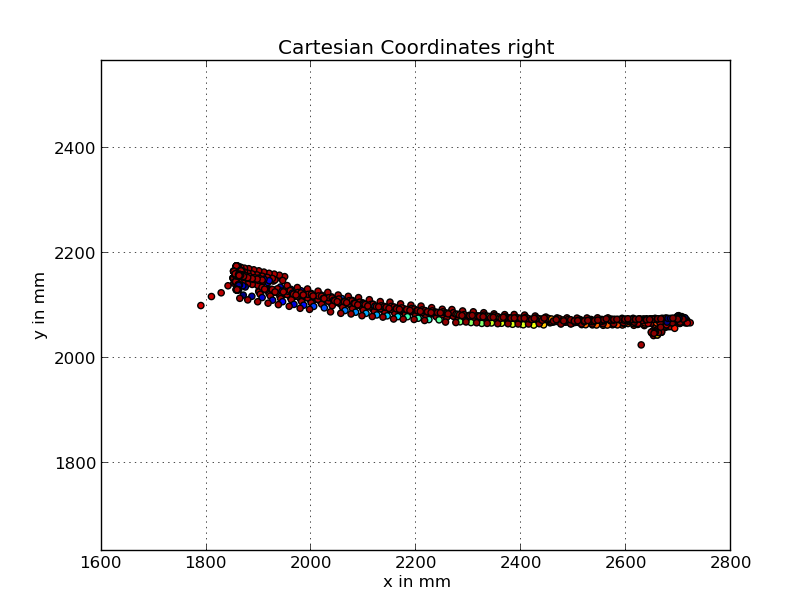
\includegraphics[width=1\linewidth]{img_second_run/Cartesian_right.png}
  %\caption{}
  %\label{fig:}
\end{minipage}%

\caption{Recordings of the right movements in cartesian coordinates.}
\label{fig:outliers}
\end{figure}


\begin{figure}[H]
\centering
\begin{minipage}{.5\textwidth}
  \centering
  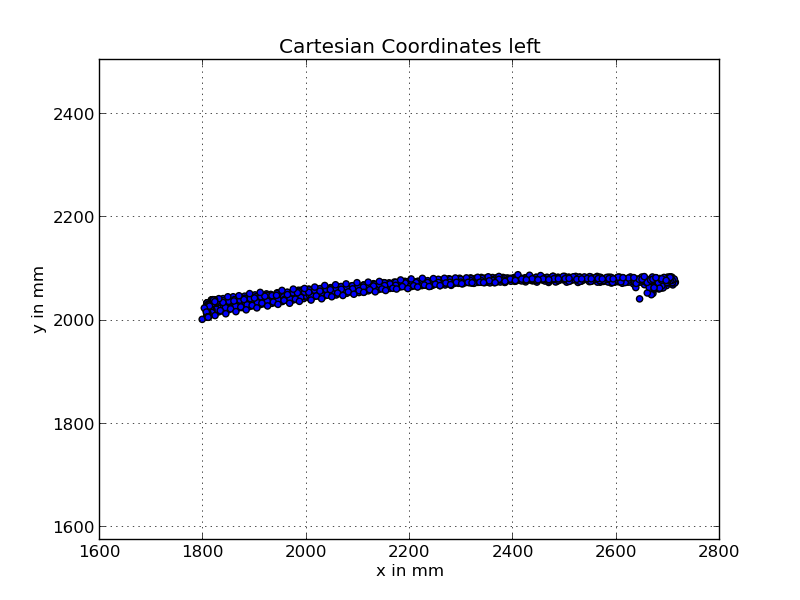
\includegraphics[width=1\linewidth]{img_second_run/Cartesian_left.png}
  %\caption{}
  %\label{fig:}
\end{minipage}%

\caption{Recordings of the left movements in cartesian coordinate}
\label{fig:outliers}
\end{figure}

To have a better understanding of the robots behaviour with respect to the commanded motions, we tried fitting two circles to the observed data of the right and left runs as suggested. Fig. 4 and Table. 1 show this observation. As depicted in the table and this figure there is an obvious trend in the robot movement towards the right side which is the reason for the smaller diameter of the right-turn circle. Removing the outliers at the ending points should expectedly reduce this difference between the two circle sizes however this doesn't resolve the issue completely. This behaviour was also observed in the previous experiments using the manual marker method so it can be due to a systematic error.\\


\begin{figure}[H]
\centering
\begin{minipage}{.5\textwidth}
  \centering
  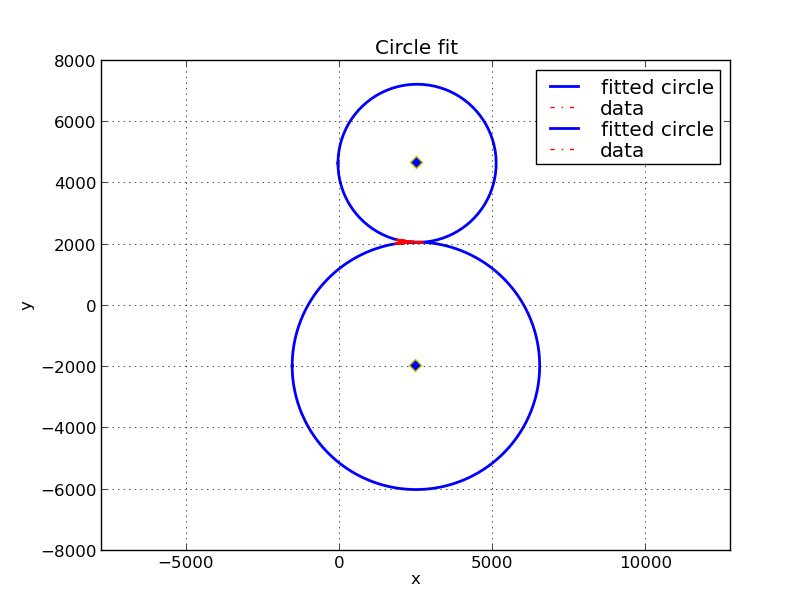
\includegraphics[width=1\linewidth]{img_second_run/Circle_fit.png}
  %\caption{}
  %\label{fig:}
\end{minipage}%

\caption{Two fitted circles for the right (upper circle) and left turns (lower circle). }
\label{fig:circles}
\end{figure}



\begin{table}[h]
\begin{tabular}{|l|l|l|l|l|}
\hline
              & xc            & yc             & R             & residu        \\ \hline
Circle\_right & 2521.4521653  & 4650.19830336  & 2582.61636419 & 96358.0886634 \\ \hline
Circle\_left  & 2483.99772597 & -1960.45625309 & 4040.6562426  & 38695.8080245 \\ \hline
\end{tabular}
\caption{Parameters and residuals of the fitted circles}
\label{my-label}
\end{table}


\section{Estimating the model parameters }

\subsection{Prediction function}
%TODO:
\begin{figure}[H]
\begin{lstlisting}[language=Python]
def predict_alphas(arg, kv=1.0, kw=1.0, bv=0.0, bw=0.0):
    x, y, theta, v, w, t, steps = arg
    d = {
        'x':x,
        'y':y,
        'theta':theta
        }
    r = [d]
    for _ in range(steps):

        #ALPHAS
        v = kv * v + bv
        w = kw * w + bw

        dv = v * t/steps
        dvx = np.cos(theta) * dv
        dvy = np.sin(theta) * dv

        dw = w * t/steps
        dwx = np.cos(theta+pi/2.0) * dw
        dwy = np.sin(theta+pi/2.0) * dw

        dx = dwx + dvx
        dy = dwy + dvy

        dtheta = np.tan(dv/dw)

        theta = theta + dtheta

        x = x + dx
        y = y + dy

        d = {
            'x':x,
            'y':y,
            'theta':theta
            }

        r.append(d)
    return r
\end{lstlisting}

\caption{Te prediction function.}
\label{fig:prediction}
\end{figure}

The prediction function takes as an input the current pose, the linear and angular velocity as well as the time it runs and the number of steps to produce during the run as the $arg$ argument. Relevant for the optimization are the scaling and biasing parameters to the angular and linear $kv$, $bv$, $kw$   and  $bw$(alphas). With those it increments with the given fraction of the time interval and updates the position x and y and the orientation theta. Based on the theta, the angular and linear velocities are broken into deltas with respect to the global x and y coordinates. The theta is updated according to its old value and the fraction of the velocities which define the angular increment.\\

With the neutral alphas 1.0 for the scaling ad 0.0 as the bias, the prediction function was run on all points of the recordings.
Figures 6 to 8 represent the distribution based on the prediction function. As observed the predicted poses don't fit completely to the observed data.

\begin{figure}[H]
\centering
\begin{minipage}{.5\textwidth}
  \centering
  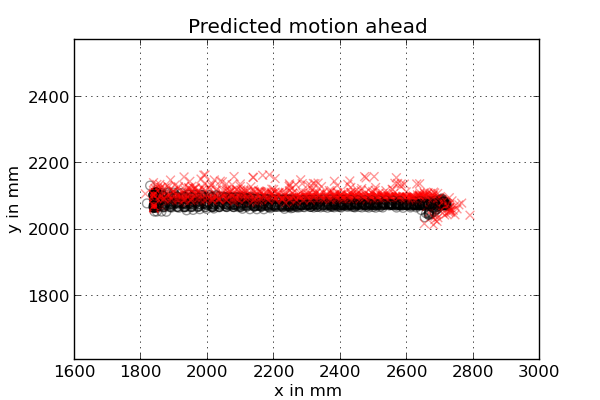
\includegraphics[width=1\linewidth]{img/predictahead.png}
  %\caption{}
  %\label{fig:}
\end{minipage}%

\caption{Results of the prediction function for forward motion. Circles mark the observations and crosses the prediction.}
\label{fig:prediction}
\end{figure}

\begin{figure}[H]
\centering
\begin{minipage}{.5\textwidth}
  \centering
  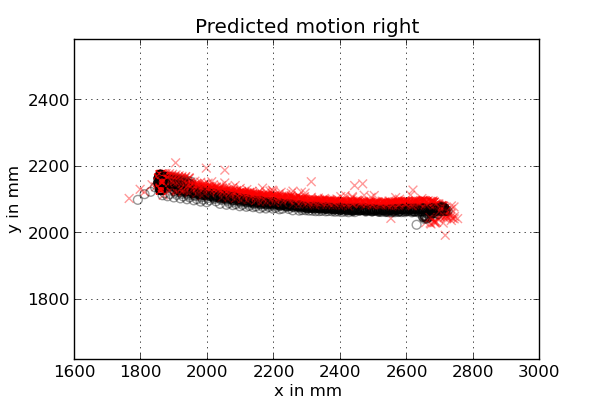
\includegraphics[width=1\linewidth]{img/predictright.png}
  %\caption{}
  %\label{fig:}
\end{minipage}%

\caption{Results of the prediction function for right turn. Circles mark the observations and crosses the prediction.}
\label{fig:prediction}
\end{figure}

\begin{figure}[H]
\centering
\begin{minipage}{.5\textwidth}
  \centering
  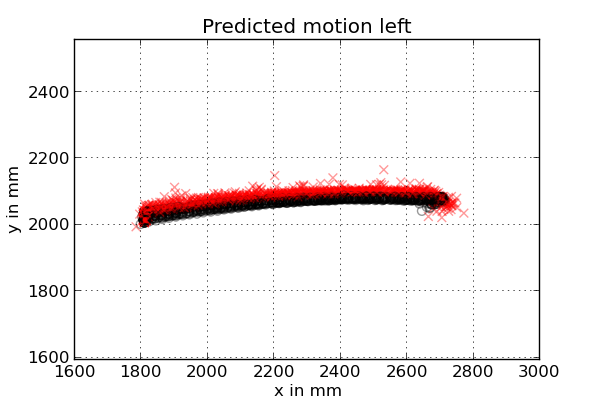
\includegraphics[width=1\linewidth]{img/predictleft.png}
  %\caption{}
  %\label{fig:}
\end{minipage}%

\caption{Results of the prediction function for left turn. Circles mark the observations and crosses the prediction.}
\label{fig:prediction}
\end{figure}

\subsection{Optimization}

%how the starting values were guessed?
Since the prediction with neutral alphas already reasonably fit the observations, the neutral alphas where chosen as starting positions for the optimization.

The starting values of motion parameters optimization and their final values after the iterative error minimization procedure can be observed in modelfit.out and also in table 2. 


%how many iterations needed for the correct fit?
We choose scipys $leastsq$ function for optimizing multiple sets of $v, w$ combinations and reached the final alphas after 435 runs.
\begin{lstlisting}[language=Python]
alphas, R =  leastsq(func = minime, x0 = (1.0, 1.0, 0.0, 0.0), args=(x, y))
kv, kw, bv, bw = alphas
\end{lstlisting}
The function to minimize calculated the mean squared error between the predictions and the observed poses.

%what is exactly the final optimized motion model?
As seen in table 2, the final prediction function is:\\
$v_{eff}=0.2033 * v + 3.0351e-05$ and $w_{eff} = 0.0204*w + 2.1060e-05$
 

\begin{table}[h]
\begin{tabular}{|l|l|l|l|l||l|}
\hline
                          & kv             & kw             & bv                & bw & mse            \\ \hline
optimization start values & 1.0 & 1.0 & 0.0 &  0.0 & 357.75        \\ \hline
final values              & 0.2033 & 0.204 & 3.0351e-05 & 2.1060e-05 & 183.89\\ \hline
\end{tabular}
\caption{Initial guesses of the motion parameters (alpha) and their final values including the mean squared error after optimization.}
\label{Motion parameters}
\end{table}

Figures 9 to 11 depict the results of the optimized motion model. As represented the motion model after removal of systematic errors, efficiently describes the observed trajectories. 

\begin{figure}[H]
\centering
\begin{minipage}{.5\textwidth}
  \centering
  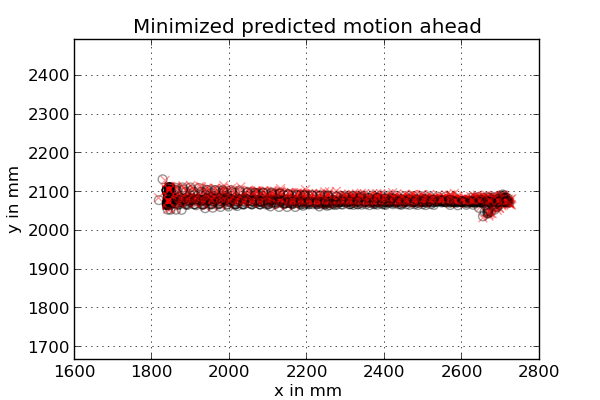
\includegraphics[width=1\linewidth]{img/mini_predict_ahead_1.png}
  %\caption{}
  %\label{fig:}
\end{minipage}%

\caption{Results of the optimized prediction function for forward motion. Circles mark the observations and crosses the prediction.}
\label{fig:prediction}
\end{figure}

\begin{figure}[H]
\centering
\begin{minipage}{.5\textwidth}
  \centering
  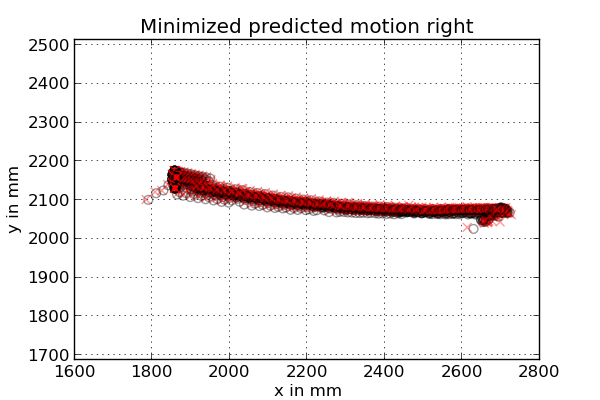
\includegraphics[width=1\linewidth]{img/mini_predict_right_1.png}
  %\caption{}
  %\label{fig:}
\end{minipage}%

\caption{Results of the optimized prediction function for forward motion. Circles mark the observations and crosses the prediction.}
\label{fig:prediction}
\end{figure}

\begin{figure}[H]
\centering
\begin{minipage}{.5\textwidth}
  \centering
  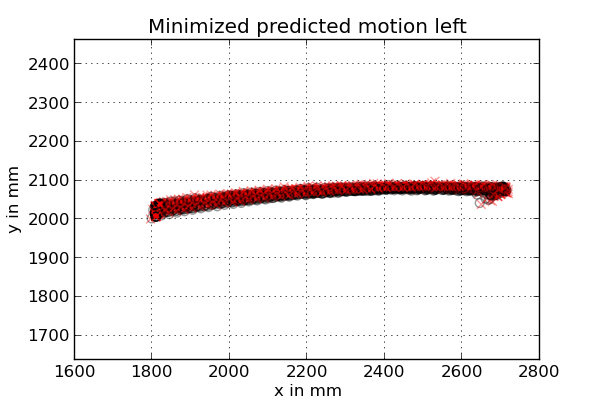
\includegraphics[width=1\linewidth]{img/mini_predict_left_1.png}
  %\caption{}
  %\label{fig:}
\end{minipage}%

\caption{Results of the optimized prediction function for forward motion. Circles mark the observations and crosses the prediction.}
\label{fig:prediction}
\end{figure}






\section{Appendix}
\subsection{Alpha values}
See modelfit.out
\lstinputlisting[linerange={1-7}]{modelfit.out}
\dots
\lstinputlisting[linerange={440-447}]{modelfit.out}




\subsection{Code}
For a complete view see \href{https://github.com/ChrisQuignon/SEE/tree/master/Homework04}{github.com/ChrisQuignon/SEE}\\
%For the trajectories please see new\_graphics.py\\
%\subsubsection{new\_graphics.py}
%\lstinputlisting[language=python]{new_graphics.py}
For the motion model approximation and circle fit please see model\_fit.py \\
%\subsubsection{model\_fit.py}
\lstinputlisting[language=python]{model_fit.py}



%BIBLIOGRPAHY!
\bibliographystyle{plain}%amsalpha
\bibliography{bib.bib}
%\bibentry{}


%COPY AND PASTE FROM HERE

%\begin{enumerate}
% \item
%\end{enumerate}

%\href{link}{text}

%\begin[Language=Python]{lstlisting}
%#PYTHON CODE HERE
%\end{lstlisting}

%\lstinputlisting[language=Java]{ }

%\csvautotabular[separator=semicolon]{data.csv}

%\begin{figure}
% \center
% \includegraphics[width= cm]{img/ }
% \caption{}
%\end{figure}



\end{document}
